\documentclass[]{article}
\usepackage{graphicx}
\usepackage{hyperref}
\usepackage{amsmath}
\usepackage{caption}
\usepackage{subcaption}
\usepackage{ngerman}
\usepackage[utf8]{inputenc}
\usepackage{float}

%opening
\title{Balmer Series}
\author{Gunther T\"urk, Jonas Lehnen}

\begin{document}

\maketitle
\begin{abstract}
Mit diesem Experiment soll das Verständnis und der Umgang mit einem Monochromator geübt werden. Dies wird anhand der Spektrallinien von Natrium, Zink und einer Wasserstofflampe durchgeführt. Die Kalibration des Monochromators, inklusive der Bestimmung der Konstante c, wird dazu genutzt um die Rydbergkonstante für Wasserstoff und Deuterium zu bestimmen. Damit werden auch die grundlegenden Annahmen des Bohr'schen Atommodels bestätigt.

\end{abstract}

\tableofcontents

\newpage
\section{Theorie}
\subsection{Bohr Modell}
Der klassische Ansatz ein Atom zu beschreiben ist ungenügend. Normalerweise würde man ein durchgängiges Spektrum an Strahlung erwarten, da der Abstand zwischen Kern und Elektron zunächst nicht beschränkt ist. Das Gegenteil wird jedoch gemessen. Ebenso sollte von einer bewegten Ladung Strahlung emittiert werden, dies geschieht im Atom jedoch nur wenn sich der Abstand verkleinert. Dies bewegte Bohr 1913 dazu seine Postulate zu formulieren. Darin beschreibt er, dass das Elektron den Kern umkreist und durch die elektrostatische Kraft auf seiner Umlaufbahn gehalten wird ohne dabei Strahlung auszusenden. Diese Bahnen werden durch ihren Drehimpuls $l = pr = n\hbar$ beschrieben. Hier bei beschreibt $n$ die Ordnung der Bahn, auch Hauptquantenzahl genannt. Zuletzt entspricht die Energie des emittierten bzw. absorbierten Photons dem Energieunterschied des Elektrons auf verschiedenen Umlaufbahnen $ \hbar \omega = E_2 - E_1$. 

Generell erhält man aus der Behandlung der Schrödingergleichung dieselbe Energie für verschiedenen $n$, welche auch aus der Gleichsetzung von Coulomb- und Zentripetalkraft folgt. $R_\infty$ wird auch Rydbergkonstante genannt. 
\begin{equation}\label{eq:Energieniveaus_H}
E_n = -\frac{1}{2} m_0 c^2 \alpha^2 \frac{Z^2}{n^2} = -13.6eV \cdot \frac{Z^2}{n^2} \: ; \: \alpha = \frac{e^2}{4\pi\epsilon_0 \hbar c} = \frac{1}{137}
\end{equation}
\begin{equation}\label{eq:rydberg}
\frac{1}{\lambda} = R_\infty \left(\frac{1}{n^2} - \frac{1}{m^2} \right)  = 10\,973\,731{,}568\,508 m^{-1} \cdot \left(\frac{1}{n^2} - \frac{1}{m^2} \right)
\end{equation}
Dadurch können wir nun die Photonenenergie bestimmen, wenn ein Elektron seinen Bahn ändert. Im folgenden sowie bereits in der zweiten Gleichung behandeln wir das Wasserstoff Atom mit $Z=1$.Hierbei wird in verschiedene Serien unterschieden, je nachdem in welche das Elektron landet, nach Photon-Emission. Jede Serie wurde nach Entdecker benannt. Die ultravioletten Spektrallinien der Lyman (Ly) Serie $Ly_\alpha \:,\: Ly_\beta \:,\: Ly_\gamma \:,\: ...$ besitzt als Grundniveau den Zustand $n=1$. Analog wurden auch die infraroten Serien Brackett (B) $n=4$ und Paschen (Pa) $n=3$, sowie die sichtbare Balmer (H) Serie $n=2$ entdeckt. 
Die lateinische Nomenklatur beschreibt von wie vielen Niveaus oberhalb, auch states genannt, das Elektron auf das Endniveau gefallen ist. Die Anzahl wird mit den Buchstaben gleichgesetzt. So hei"st der \"Ubergang $5 \rightarrow 2$ auch $B_\gamma$.

\subsection{Ebert Monochromator}
Um das Licht eines Elements analysieren zu können müssen wir die Spektrallinien auffächern. Hier im Experiment wird dies mit einer Form des Ebert Monochromators umgesetzt. Dabei handelt es sich um um zwei  Spalte durch die das Licht ein- und ausfallen kann. Während dem Durchgang wird der Lichtstrahl zwischen zwei Reflexionen an einem Hohlspiegel auch an einem Gitter umgelenkt. Dieses Gitter ist nun drehbar und der Winkel $\delta$ in  Abbildung \ref{fig:Monochromator} bezeichnet die Verstellung bezüglich der parallel Lichtstrahlen. 

\begin{figure}[H]
\centering
\begin{subfigure}{0.55\textwidth}
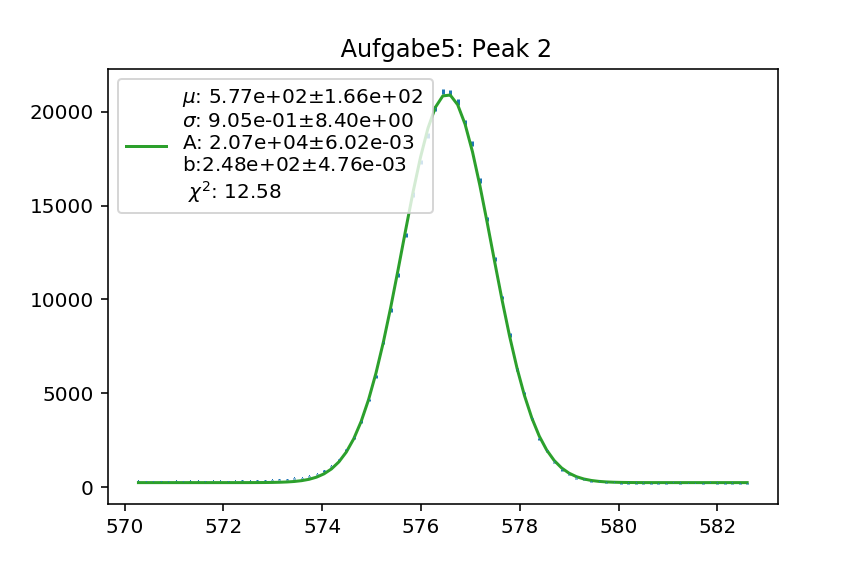
\includegraphics[width=\linewidth]{Plots/1.png}
\end{subfigure}
\begin{subfigure}[c]{0.4\linewidth}
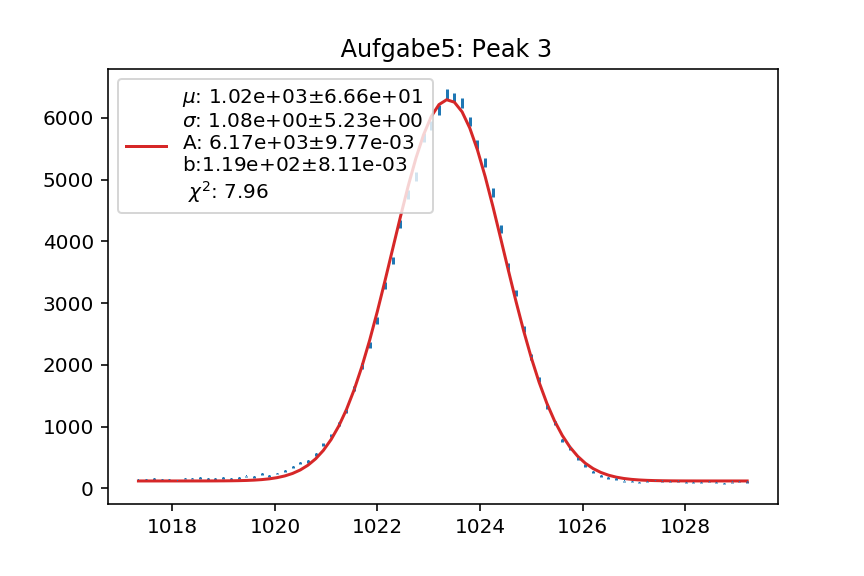
\includegraphics[width=\linewidth]{Plots/2.png}
\end{subfigure}
\caption{Schematische Darstellung eines Ebert Monochromators. Grafiken wurden dem zum Experiment mitgegebenen Skript (SS 2006) entnommen. }
\label{fig:Monochromator}
\end{figure}

Durch das drehbare Gitter erhält man trotz konstantem Strahlengang, welcher durch die festen Positionen der Spalte gegeben ist, eine Änderung im Laufweg des Lichts, je nach Wellenlänge. Diesen Unterschied erkennt man, wenn man wie im späteren Einzelspalt die verschiedenen Maxima betrachtet. 

% SKIZZE einfügen für den Strahlengang im Gitter + Herleitung
So erhält man aus Abbildung <<<ref>>> folgende Bedingung an Gangunterschied bei konstruktiver Interferenz:
\begin{align}
\Delta &= g\cdot sin(\beta) + g\cdot sin(\gamma) = g\cdot \left( sin(\delta - \alpha) + sin(\delta + \alpha)  \right) \\
 &= g\cdot ( sin(\delta)cos(\alpha) + cos(\delta)sin(\alpha) +  sin(\delta)cos(\alpha) - cos(\delta)sin(\alpha) ) \\
 &= 2g \cdot cos(\alpha) sin(\delta) =: c \cdot sin(\delta) \stackrel{!}{=} n\lambda \label{eq:c sin = n lam}
\end{align}

Diese Beziehung wird in der Auswertung unserer Messwerte benutzt um zunächst c durch die Natrium und Zink Daten zu bestimmen. Später, beim Wasserstoff wird Gleichung (\ref{eq:c sin = n lam}) genutzt um die Wellenlängen und damit auch die Rydbergkonstanten zu bestimmen.

\subsection{Quantenmechanik}
\subsubsection{Schrödingergleichung}
Während das Bohrsche Atommodell in der Lage ist die Spektrallinien von Wasserstoff vorherzusagen, so versagt es doch bei der Erklärung der Fein- und Hyperfeinstruktur, sowie der Vorhersage von Spektrallinien bei Atomen mit mehr als einem Elektron. Aus der 1927 nachgewiesenen de Broglie Beziehung zwischen Impuls und Wellenlänge $ \lambda=\frac{h}{p} $ wobei h das Plank'sche Wikrungsquantum ist und der aus dem Photoeffekt bekannten Beziehung $ E=hf=\hbar \omega $ kann man die Schrödingergleichung motivieren. In der Quantenmechanik beschreibt man Teilchen mithilfe von Wellenfunktionen. Dabei beschreibt man ein freies Teilchen als ebene Welle.
\begin{equation}
\Psi(\vec{x},t)=A e^{i(k \vec{x}-\omega t)}
\end{equation} 
Als erstes betrachten wir die Zeit- und Ortsableitung dieser ebenen Welle. 
\begin{equation}
\label{eq:Energie} \frac{\partial}{\partial t} \Psi(\vec{x},t)=(-i\omega)  \Psi(\vec{x},t)=-\frac{iE}{\hbar} \Psi(\vec{x},t) \Rightarrow i\hbar \frac{\partial}{\partial t}=E  \Psi(\vec{x},t) \end{equation}
\begin{equation}
\label{eq:Impuls} \nabla  \Psi(\vec{x},t) =i\vec{k} \Psi(\vec{x},t)=\frac{i\vec{p}}{\hbar} \Psi(\vec{x},t) \Rightarrow -i\hbar \nabla  \Psi(\vec{x},t)= \vec{p}    \: \Psi(\vec{x},t) \end{equation}
Aus der klassischen Mechanik wissen wir, dass die Energie eines Teilchens \begin{equation} E=T+V=\frac{\vec{p}^2}{2\mu}+V(\vec{x}) 	\end{equation} wobei $\mu$ die reduzierte Masse ist. Um daraus eine quantenmechanische Beschreibung zu erhalten muss man den Impuls nach Gl. \ref{eq:Impuls} als $-i\hbar \nabla$ schhreiben und die Energie als $i \hbar \frac{\partial}{\partial t}$ schreiben und die Gleichung mit $\Psi(\vec{x},t)$ multiplizieren. Daraus erhält man dann 
\begin{equation}
\label{eq:Schrodinger}
i\hbar \frac{\partial}{\partial t}\Psi(\vec{x},t)=(-\frac{\hbar^2}{2\mu}\nabla^2+V(\vec{x})) \Psi(\vec{x},t) 
\end{equation}
was die Schrödingergleichung ist.
\subsubsection{Das Wasserstoffatom}
Um jetzt die gebundenen Energiezustände des Wasserstoffatoms zu berechnen und damit dann die $\delta E$ der Spektrallinien zu erhalten muss man die Schrödingergleichung für ein Potential
\begin{equation}
	V(r)=\frac{-e^2}{4\pi \epsilon} \frac{1}{r}
\end{equation}
lösen, also die Welleneigenfunkionen bestimmen. Da diese Rechnung in jedem Buch zur Quantenmechanik gefunden werden kann sparen wir uns hier die ausführlichen Rechnungen und Ergebnisse. Für unsere Zwecke reicht es zu wissen, dass die Energieniveaus $E_{n}$ gegeben sind durch
\begin{equation}
\label{eq:Wasserstoff}
	E_{n}=\frac{-e^4\mu}{8\epsilon_0^2h^2}\cdot \frac{1}{n^2}=-\frac{\mu c^2}{2}\frac{\alpha^2}{n^2}
\end{equation} und wir aus der Lösung der Gleichung zwei weitere Quantenzahlen l,m erhalten, wobei l=0,1,2,...,n-1 den Drehimpuls quantifizieren und m=-l,(-l+1),...(l-1),l m die magnetische Quantenzahl ist. Die Energiewerte sind in l und m entartet, da diese die Energie für ein gegebenens n nicht ändern.
\subsubsection{Feinstruktur}
Die Entartung der Energiewerte aus Gl. \ref{eq:Wasserstoff} wird in l aufgehoben, wenn man die Korrekturen der Feinstruktur betrachetet. Dabei berücksichtigt man die relativistische Massenkorrektur des Elektrons sowie die Spin-Bahn-Kopplung des magnetischen Moments des Elektrons an seine Bahn. Außerdem kommt noch der Darwin-Term hinzu den man nicht durch Störungsrechnung motivieren kann, sondern ein Ergebnis der relativistischen Behandlung des Wasserstoffatoms mit der Dirac-Gleichung ist. 
Für unser Experiment können wir jedoch die Korrekturen an die Schrödingergleichung durch die Feinstruktur vernachlässigen, da sie um den Faktor $\alpha^2 \approx  10^{-4}$ unterdrückt sind und damit zu klein sind für die Auflösung unseres Experiments. Die Korrekturen der Hyperfeinstruktur $\sim \alpha^4$ sind natürlich auch irrelevant für uns, weshalb wir nicht weiter auf sie eingehen.
%%Hier müssen die korrekturterme hin. und noch etwas beschriebung der LS kopplung 
%Na doppellinie"
\subsection{Beugung und Interferenz} %Neu schreiben mit es Photonen als anfang und dann welleneigenschaften
Interferenz und Beugung sind Phänomene die nur bei Wellen beobachtet werden. Die Überlegungen von de Broglie zur Materie-welle und der Beweis des Teilchencharakters von Photonen beschreiben die gleichzeitige Existenz eines Teilchens als Welle. Dies wird dann in der Quantenmechanik mathematisch Beschrieben. 
\subsubsection{Einfachspalt}
Fällt Licht auf einen einzelnen Spalt, so detektiert man dahinter nicht eine Normalverteilung der Intensität um die mitte des Spalts, sondern ein Interferenzmuster(Abb (\ref{fig:?????})). Insbesondere die Nebenmaxima lassen sich nicht mit klassischen Überlegungen erklären, da dieses Muster auch dann auftritt, wenn man einzelne Photonen durch den Spalt schickt und diese deshalb nicht miteinander Interferieren können.%Hier könnte man den klugscheißerkommentar anbringen vonwegen eichtheorie bla bla bla
Die Frage ist jetzt wie dieses Muster entstehen kann wo es doch nicht also Bewegung der Photonen aufgrund einer Bewegungsgleichung beschrieben wird. Betrachten wir das Photon als Teilchen, dass eine Wahrscheinlichkeitsdichte $\Psi(x)$ hat, dass sich auf den Spalt zubewegt, können wir es beschreiben als 
\begin{equation}
	Psi(x)=\Psi_{0}e^{i(kx-\omega t)}
\end{equation}
Der Einfachheit halber betrachten wir das Ganze nur in einer Dimension. Nach dem Fresnel'schen Prinzip entsteht an jedem Auftreffpunkt des Spalts eine neue Kugelwelle, welche bis auf eine eventuelle Phasenverschiebung von $\delta =y sin(\alpha) $ ihrer Ursprungswelle gleicht. Dabei ist zu beachten, dass eine Kugelwelle auch eine Beugung entgegen der Bewegungsrichtung des Strahls vorausgesetzt wird, die nicht beobachtet wird. Wir machen weiterhin die Annahme der Frauenhofer Beugung, d.h. dass sich der Schirm unendlich weit weg vom Spalt befindet. Die auslaufende welle kann also beschrieben werden als
\begin{equation}
	\Psi(x)=\tilde{\Psi_{0}}e^{i(k(x-\delta)-\omega t)}
\end{equation}
Auf einem unendlich weit entfernten Schirm treffen alle Strahlen die den Spalt parallel zueinander durchquert haben am selben Punkt auf. Um die Wahrscheinlichkeitsamplitude an diesem Punkt zu berechnen integrieren wir also über alle Wellen die den Spalt unter dem selben Winkel verlassen.
\begin{align}%%%Hier muss irgendow noch ein psinull schlange hin, dass e^-ikx-wt mitnimmt
	\Psi_{Schirm}(x,\alpha)&=\underbrace{\Tilde{\Psi_{0}}e^{kx-\omega t}}_{\Psi_{0}}\frac{1}{d}\int_{-d/2}^{d/2} e^{-iky\: sin(\alpha)}  \\ 
	%
	&=-\frac{\Psi_{0}}{ikd \: sin \: \alpha} [e^{-iky \: sin(\alpha)}]^{+d/2}_{-d/2} \\
	%
	&=-\frac{\Psi_{0}}{ikd \: sin \: \alpha} \underbrace{(e^{-ik\frac{d}{2}sin(\alpha)}-e^{ik\frac{d}{2}\:sin(\alpha)})}_{-2i\: sin(k\frac{d}{2}sin \alpha))} \\
	%
	&=\Psi_{0}\frac{2}{kd\: sin \: \alpha}sin(\frac{\pi d}{\lambda}sin \: \alpha) 
\end{align}
Setzt man jetzt noch $k=\frac{2\pi}{\lambda}$ ein, so ergibt sich die relative Intensität zu
\begin{equation}
I_{relativ}=	\frac{|\Psi_{Schirm}|^2}{|\Psi_{0}|^2}=(\frac{\lambda}{\pi d \: sin \: \alpha} sin(\frac{\pi d}{\lambda} sin \: \alpha))^2
\end{equation}

Die Intensität folgt also der Funktion 
\begin{equation}
	sinc(\frac{\pi d}{\lambda} sin \: \alpha)
\end{equation} 
Hiervon können wir die lokalen Extremstellen bestimmen, was uns eine Aussage über die Lage der hellen und dunklen Streifen unseres Beugungsmusters gibt.

\begin{align}
	&Minima: &m\pi&= x \rightarrow m\pi &= \frac{\pi d}{\lambda} \: sin \: \alpha	&\Rightarrow \frac{m}{d} &=\frac{sin \: \alpha}{\lambda}\\
	%
	&Maxima: &\frac{2m+1}{2}\pi&=x \rightarrow \frac{2m+1}{2}\pi &= \frac{\pi d}{\lambda}\:sin \: \alpha &\Rightarrow \frac{2m +1}{2d}&=\frac{sin \: \alpha}{\lambda}
\end{align}
Wir stellen fest, dass die Funktion $\Psi_{Schirm}$ nichts anderes ist, als die Fouriertransformierte der Spaltfunktion mal Konstanten, wir also nur vom Orts- in den Impulsraum gewechselt sind. Sobald wir die Wellenfunktion haben, können wir die Intensität als deren Betragsquadrat einfach ausrechnen. Das erlaubt uns auch kompliziertere Beugungsmuster zu errechnen.
\subsubsection{Doppelspalt}
Die Herleitung der Intensitätsverteilung beim Doppelspalt erfolgt analog zu der beim Einfachspalt. Anstatt aber nur über den einen Spalt zu integrieren, integriert man über zwei. 
%Hier das Bild vom Doppelspalt hin
\begin{align}
	\Psi_{doppelt}(x,a)&=\Psi_{0}\frac{1}{2d}(\int_{-D/2-d/2}^{-D/2+d/2}e^{-iky \: sin \: \alpha}dy+\int_{D/2-d/2}^{D/2+d/2}e^{-iky \: sin \: \alpha}dy)\\
%
	&=-\frac{\Psi_{0}}{2idk \: sin \: \alpha}([e^{-iky \: sin \alpha}]_{-D/2-d/2}^{-D/2+d/2}+[e^{-iky \: sin \alpha}]_{D/2-d/2}^{D/2+d/2})\\
%
	&=\frac{\Psi_{0}}{2idk \: sin \: \alpha}(e^{ik\frac{D}{2} sin \: \alpha}+ e^{-ik\frac{D}{2} sin \: \alpha})(e^{-ik\frac{d}{2} sin \: \alpha}+ e^{ik\frac{d}{2} sin \: \alpha})\\
%5
	&=\Psi_{0}\frac{2}{dk \: sin \: \alpha}sin (\frac{kd}{2} sin \: \alpha)\: cos(\frac{kD}{2}sin \: \alpha)
\end{align}
mit $k=\frac{2 \pi}{\lambda}$ ergibt sie die relative Intensität zu
\begin{align}
	I_{relativ}&=	\frac{|\Psi_{doppelt}|^2}{|\Psi_{0}|^2}=\left( \frac{\lambda}{\pi d \: sin \: \alpha}sin \left(  \frac{\pi d}{\lambda} sin \: \alpha \right)\right)^2 \cdot cos^2 \left( \frac{\pi D}{\lambda}sin \: \alpha \right) 
\end{align}


Man erkennt, dass die Intensität am Doppelspalt ein Produkt aus dem Einfachspalt und dem Quadrat eines Kosinus der vom Spaltabstand D abhängt ist. Für den Normalfall, dass der Spaltabstand viel größer ist als die Spaltbreite d ist, bildet der sinc eine Einhüllende und der Kosinus ist maßgeblich für die Lage der Minima und Maxima.

\begin{align}
	&Maxima: m\pi&=\frac{\pi d}{\lambda}sin \: \alpha &\Rightarrow \frac{m}{D}&= \frac {sin \: \alpha}{\lambda } \\
	&Minima: \frac{2m+1}{2}\pi&=\frac{\pi d}{\lambda}sin \: \alpha &\Rightarrow \frac{2m+1}{2D}&=\frac{sin \: \alpha}{\lambda}	
\end{align}
Auch hier was über die lage der maxima und minmima noch hinschreiben



%Hier muss dann die Herleitung hin
\subsubsection{Beugungsgitter}
In der Praxis verwendet man anstelle eines Doppelspalts meist ein Beugungsgitter. Um die Intensitätsverteilung davon zu erhalten, können wir uns das Wissen über die Intensität vom Einzelspalt zunutze machen. Das Beugungsgitter ist eine aneinanderreihung von vielen Einfachspalten. 
\begin{equation}
f(x)=1 oder 0 je nachdem
\end{equation}
Um diese zu erhalten reicht es, die Funktion des Einfachspalts mit deiner Summe von Deltafunktionen zu falten. Wir wählen
\begin{equation}
	g(x)=\sum_{l=0}^{n-1}\delta(x-lG)
\end{equation}
wobei G der Gitterabstand ist. Die Faltung von g und f ist definiert als
\begin{equation}
	(f*g)(x)=\int_{\Re} f(y)g(x-y)dy
\end{equation}
Die Fouriertransformation der Faltung gibt uns jetzt die Wellenfunktion am Schirm. Zur Berechnung nutzen wir das Faltungstheorem aus, welches besagt, dass die Fouriertransformierte der Faltung $(f*g)(x)$ das Produkt der einzelnen Fouriertransformierten von $ f(x) $ und $ g(x) $ ist. Wir kennen bereits die Lösung für den Einzelspalt, es bleibt also nurnoch die für $g(x)$ zu berechnen.
\begin{align}
	\textit{F}(g)&=\int_{\Re}\sum_{l=0}^{n-1}\delta(x-lG)e^{ikx \ sin \ \alpha}\\
				&=\sum_{l=0}^{n-1}e^{iklG \ sin \ \alpha}\\
				&=\frac{sin(\frac{nkG}{2}sin \ \alpha)}{sin(\frac{kG}{2}sin \ \alpha)}
\end{align}

Genau wie wir beim Einfachspalt den Term $\frac{1}{d}$ bekommen, da wir über alle möglichen Wellen im Spaltabstand d integrieren müssen wir \textit{F}(g) noch durch n teilen. 
Damit folgt für $k=\frac{2\pi}{\lambda}$
\begin{equation}
	I_{relativ}=\left|\frac{F(f) }{d}\right|^2\cdot\left|\frac{F(g)}{n}\right|^2=\left(\frac{\lambda}{\pi d \ sin \ \alpha}sin \left(\frac{\pi d}{\lambda}sin \ \alpha\right)\right)^2\cdot\left(\frac{sin \left(n \pi \frac{G}{\lambda} \ sin \ \alpha \right)}{sin \left(\pi \frac{G}{\lambda} \ sin \ \alpha\right)}\right)^2
\end{equation}
Wie beim Doppelspalt bildet hier das Beugungsmuster vom Einfachspalt die Einhüllende, während das Gitter für die lokalen Peaks verantwortlich ist. Dabei liegen zwischen zwei Peaks die die Einhüllende berühren immer $n-2$ lokale Maxima. Für den Fall von $n=2$ erhält man die Intensitätsverteilung des Doppelspalts.

\begin{align}
	\Psi_{Gitter}(x,\alpha)
\end{align}


\subsubsection{Balmer Serie}
Die Übergänge im Wasserstoff von $n>3$ auf $n=2$ bezeichnet man als Balmer Serie. Die Wellenlängen dieser Übergänge lassen sich nach Gl. \ref{eq:Energieniveaus_H} einfach berechnen. Dabei sind die Wellenlängen mit m=3,4,5,6 zwischen 400nm und 700nm, also im sichtbaren Bereich. Sie sind deshalb besonders einfach nachzuweisen, da wir unser Auge als Detektor verwenden können, der sowohl die Lage als auch die Wellenlänge (Farbe) und auch qualitativ die Intensität der Übergänge bestimmen kann.
\begin{table}[H]
	\centering
	\caption{Sichtbare Übergänge der Balmer Serie}
	\label{my-label}
	\begin{tabular}{|l|l|l|l|l|}
		\hline
		Übergang von n auf m  & 3 $\rightarrow$  2 & 4 $\rightarrow$ 2 & 5 $\rightarrow$ 2 & 6 $  \rightarrow$ 2 \\ \hline
		Name                  & $H_{\alpha }$      & $H_{\beta}$        & $H_{4\gamma }$      & $_{\delta}$       \\ \hline
		Wellenlänge (nm)      & 656.285                      & 486.128                      & 434.046                       & 410.174                        \\ \hline
		Energiedifferenz (eV) & 1.89                           & 2.55                           & 2.86                           & 3.03                           \\ \hline
		Farbe                 & Rot                            & Aquamarin                      & Blau                           & Violett                        \\ \hline

	\end{tabular}
\end{table}


\subsection{Isotopenshift}
Bei der Herleitung der Energieniveaus aus dem Bohr Modell haben wir angenommen, dass der Atomkern eine unendliche Masse hat. Um die Masse zu berücksichtigen, können wir wie in der klassischen Mechanik das Problem im Schwerpunktsystem betrachten. Das einzige was sich in der Gleichung ändert ist, dass wir statt $m_0$ die relative Masse 
\begin{equation}
	\mu=\left(\frac{1}{m_{p^+}}+\frac{1}{m_{e^-}}  \right)= \frac{m_1 m_2}{M}
\end{equation}
in die Gleichung \ref{eq:rydberg} einsetzen. Da wir in unserer Wasserstofflampe Wasserstoff und Deuterium in einem Verhältnis von 9/1 haben erhalten wir bei jeder Spektrallinie der Balmer Serie je eine für Wasserstoff und eine für Deuterium, die sehr nah beieinander liegen und sich oft überlagern. Damit können wir das Auflösungsvermögen unserer Apparatur bestimmen.




\newpage
\section{Experiment}
\subsection{Setup}

Hier im Experiment wird ein Ebert Monochromator benutzt wie er auch schon in der Theorie beschrieben wurde. Der Aufbau wurde durch einen justierbaren Spiegel über dem Gitter erweitert. Der Spiegel ist verbunden mit der Gitterachse und dreht sich somit mit wenn der Winkel verändert wird. Dadurch wird zusätzliches Licht, das auf den Spiegel geworfen wird auf ein Maßband reflektiert. Dieses Maßband wurde in einem $90^\circ$ Winkel angebracht. Der Abstand zwischen Spiegel und Maßband wurde folgendermaßen ermittelt:

\begin{table}[H]
	\centering
	\begin{tabular}{c|c|c|c|c|c}
		Messung & 1 & 2 & 3 & 4 & Mittelwert \\
		\hline
		Abstand r [cm] & 250 & 250.5 & 250 & 250.5 & 250.25 $\pm$ 0.25 \\
	\end{tabular}
	\caption{Gemessene Abstände zwischen Spiegel und Maßband.}
\end{table}

Die folgenden Gleichungen (\ref{eq:Umrechnung Winkel}) beschreiben die Umrechnung vom gemessenen Abstand x auf dem Maßband zum Gitterstellung, beschrieben durch den Winkel $\delta$. Der Faktor $\frac{1}{2}$ entsteht durch die Übersetzung vom eigentlichen Gitter im Monochromator zum Spiegel obenauf.
\begin{equation}\label{eq:Umrechnung Winkel}
\delta= \frac{1}{2}\frac{x}{r} \cdot \frac{180^\circ}{\pi} \:,\: \Delta\delta= \frac{1}{2} \sqrt{\left(\frac{\Delta x}{r}\right)^2 + \left(\frac{x\cdot \Delta r}{r^2}\right)^2} \cdot \frac{180^\circ}{\pi}
\end{equation}

Die der Inhalt Wasserstofflampe, welche zur Aufnahme der Balmer Serie benutzt wird, bestanden zu $90\%$ aus $H_2O$ und $10\%$ $D_2O$, sodass für höhere Ordnungen der Isotopenshift erwartet wird. Ebenso erwarten wir nicht nur die Spektrallinien von Wasserstoff H und Deuterium D aufzunehmen, sondern auch Linien vom Sauerstoff, da in der Lampe bei der (Wasser-)Elektrolyse neben $H_2$ auch $O_2$ zu erwarten ist.


\subsection{Auswertung}
\subsubsection{Natrium Doppellinien}

\subsubsection{Zink Spektrallinien}
Nach dem Wechsel zur Zink Lampe wurden erneut die 4m des Maßbandes abgefahren um nach Spektrallinien zu suchen. Abbildung \ref{fig:Zink} veranschaulicht die gefundenen Linien. Man erkennt sehr schön die erwarteten vier Linien pro Ordnung. Die farbliche Reihenfolge jeder Ordnung beleibt auch stets konstant jedoch beginnt die 4. Ordnung bereits bevor die Dritte abgeschlossen ist. Wir konnten vier komplette Ordnungen vermessen und die ersten zwei Linien der Fünften. Ebenso ist es deutlich geworden, dass, wie erwartet, mit zunehmender Ordnung der Anstand zwischen den Spektrallinien deutlich zunimmt. 

Interessant sind vor allem die Winkel ab ca. $45^\circ$. Man erkennt sehr deutlich wie stark sich nun die 4. Ordnung durch die rote Linie ausdehnt und nun sogar den Anfang der 5. Ordnung überholt hat. Seltsam ist es, dass die olivfarbene Linie zum Schluss nicht mehr zu sehen ist. Trotz der zunehmenden Abstände und dem besseren Auflösungsvermögen in n, sollte sie noch nicht außerhalb der aufgenommenen Daten sein. Man könnte den dreifachen Abstand zwischen violett und blau erwarten, jedoch wurde dort nichts gesehen. Die lässt auf den erwarteten Verlust der Intensität schließen, wie er auch noch in den Grafiken zum Wasserstoff sichtbar ist, Abbildungen \ref{fig:H Lines 0} und \ref{fig:H Lines 1}.

\begin{figure}[H]
\centering
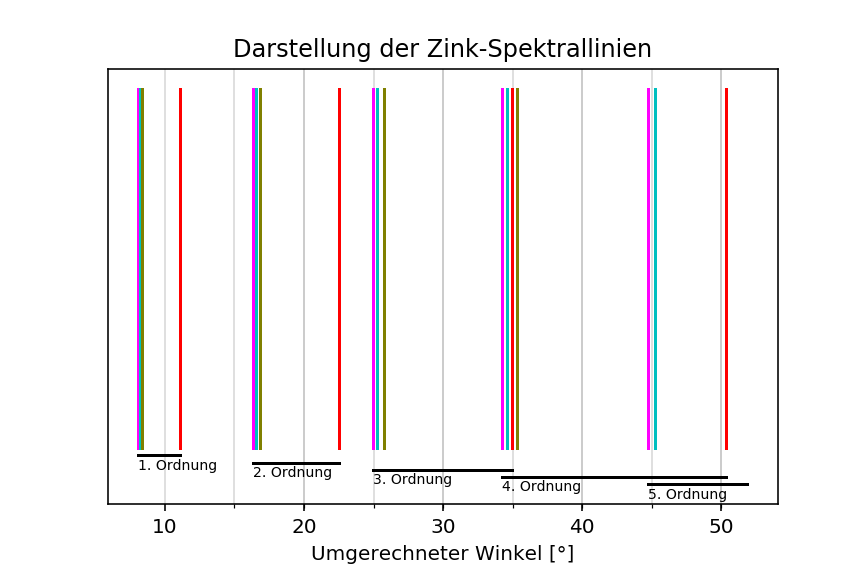
\includegraphics[width=.9\linewidth]{Plots/Zink_Linien.png}
\caption{ Grafische Darstellung des Zinkspektrums inkl. zugewiesenen Ordnungen der Maxima. Für exakte Daten siehe Anhang: Tabelle \ref{Zn Data} }
\label{fig:Zink}
\end{figure}

\begin{table}[H]
	\centering
	\begin{tabular}{c|c|c|c|c}
		Farbe & violett & blau & oliv  & rot \\
		\hline
		Wellenlänge [nm]  & 468.0 & 472.2 & 481.1 & 636.2 \\
	\end{tabular}
	\caption{Theoretische Werte für die Spektrallinien von Zink. Diese Werte werden auch zur Bestimmung vom c benutzt und entstammen dem Skript \cite{skript}.}
\end{table}

\subsubsection{Monochromatorkonstante}
Die Monochromatorkonstante c ist essentiell für diesen Versuch, damit wir später die Rydbergkonstante bestimmen  können. Zunächst betrachten wir die theoretische Bestimmung von c. Durch die aus dem Skript gegebenen Werte von Abstand zwischen den Spalten und ihrem Auftreffpunkt am Hohlspiegel F, dem Abstand zwischen diesen Auftreffpunkten 2R und dem Abstand zwischen Gitter und den Spalten D, können wir nun c bestimmen. 

\begin{align}
F&= 400mm ,\: D= 59mm ,\: R=30mm \:\: sowie \: Gitterkonstante \: g=\frac{1mm}{600} \\
c&= 2g\: cos(\alpha) = 2g\: \frac{F-D}{\sqrt{(F-D)^2 + R^2}} = 3320.5\:nm
\end{align}

Diesen Wert vergleichen wir nun mit den Ergebnissen, welche aus den Daten der Natrium-Doppellinien und den Zink Spektrallinien erhalten. Wie es bereits in der Theorie dargestellt wurde tragen wir $sin(\delta)$ gegen die Wellenlänge gewichtet mit der Ordnung des Maximums $n\cdot\lambda$ auf, siehe Abbildung \ref{fig:MonoConst}.

\begin{figure}[H]
\centering
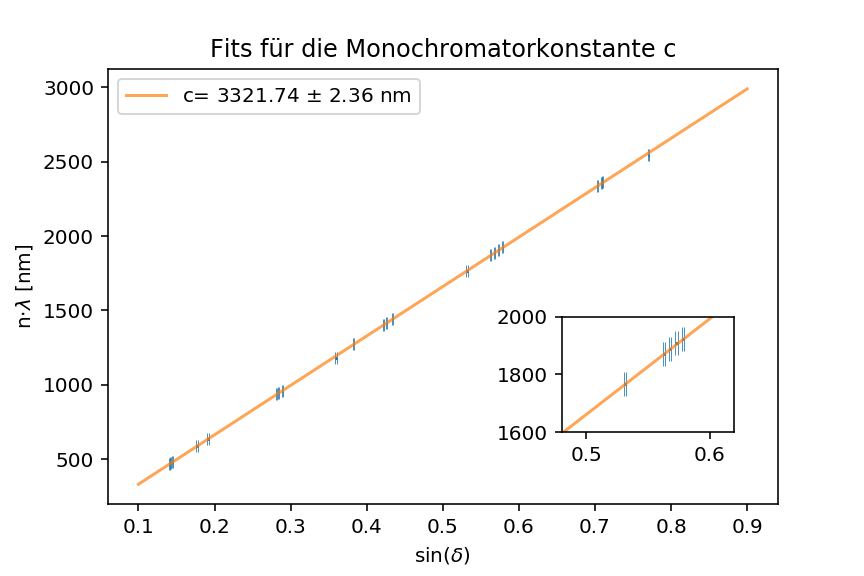
\includegraphics[width=.9\linewidth]{Plots/Monochromatorkonstante.png}
\caption{Bestimmung der Monochromatorkonsante durch einen linearen Fit. Gewichtung des Fits mit Fehlern auf den gemessenen Winkel $\delta$. Zoom zur Veranschaulichung der einzelnen Datenpunkte. Wellenlängen wurden aus dem Skript zum Versuch \cite{skript} entnommen. Weitere Werte siehe Anhang, Tabelle \ref{c Data}. }
\label{fig:MonoConst}
\end{figure}

Das Resultat aus dem linearen Fit $c = 3321.74 \pm 2.36 \: nm$ entspricht innerhalb seines Fehlers genau dem Wert aus den gegebenen Werten. Mit dieser Übereinstimmung von ca. $99.96\%$ zum geometrischen Ergebnis kann man mit guten Gewissen im folgenden diesen Wert zur Bestimmung der Rydbergkonstanten benutzen.

\subsubsection{Spektrum einer Wasserstofflampe}
Zuletzt wurde das Spektrum der Wasserstofflampe aufgenommen. Zur besseren Übersicht wurde die Grafik in zweit Teile geteilt, siehe Abbildungen \ref{fig:H Lines 0} und \ref{fig:H Lines 1}. An der Teilungsstelle wurde auch der Spiegel zur Datenaufnahme neu justiert. Die schwarzen Linien indizieren wieder wie weit sich eine Ordnung erstreckt und sind absteigend dargestellt.

\begin{figure}[H]
\centering
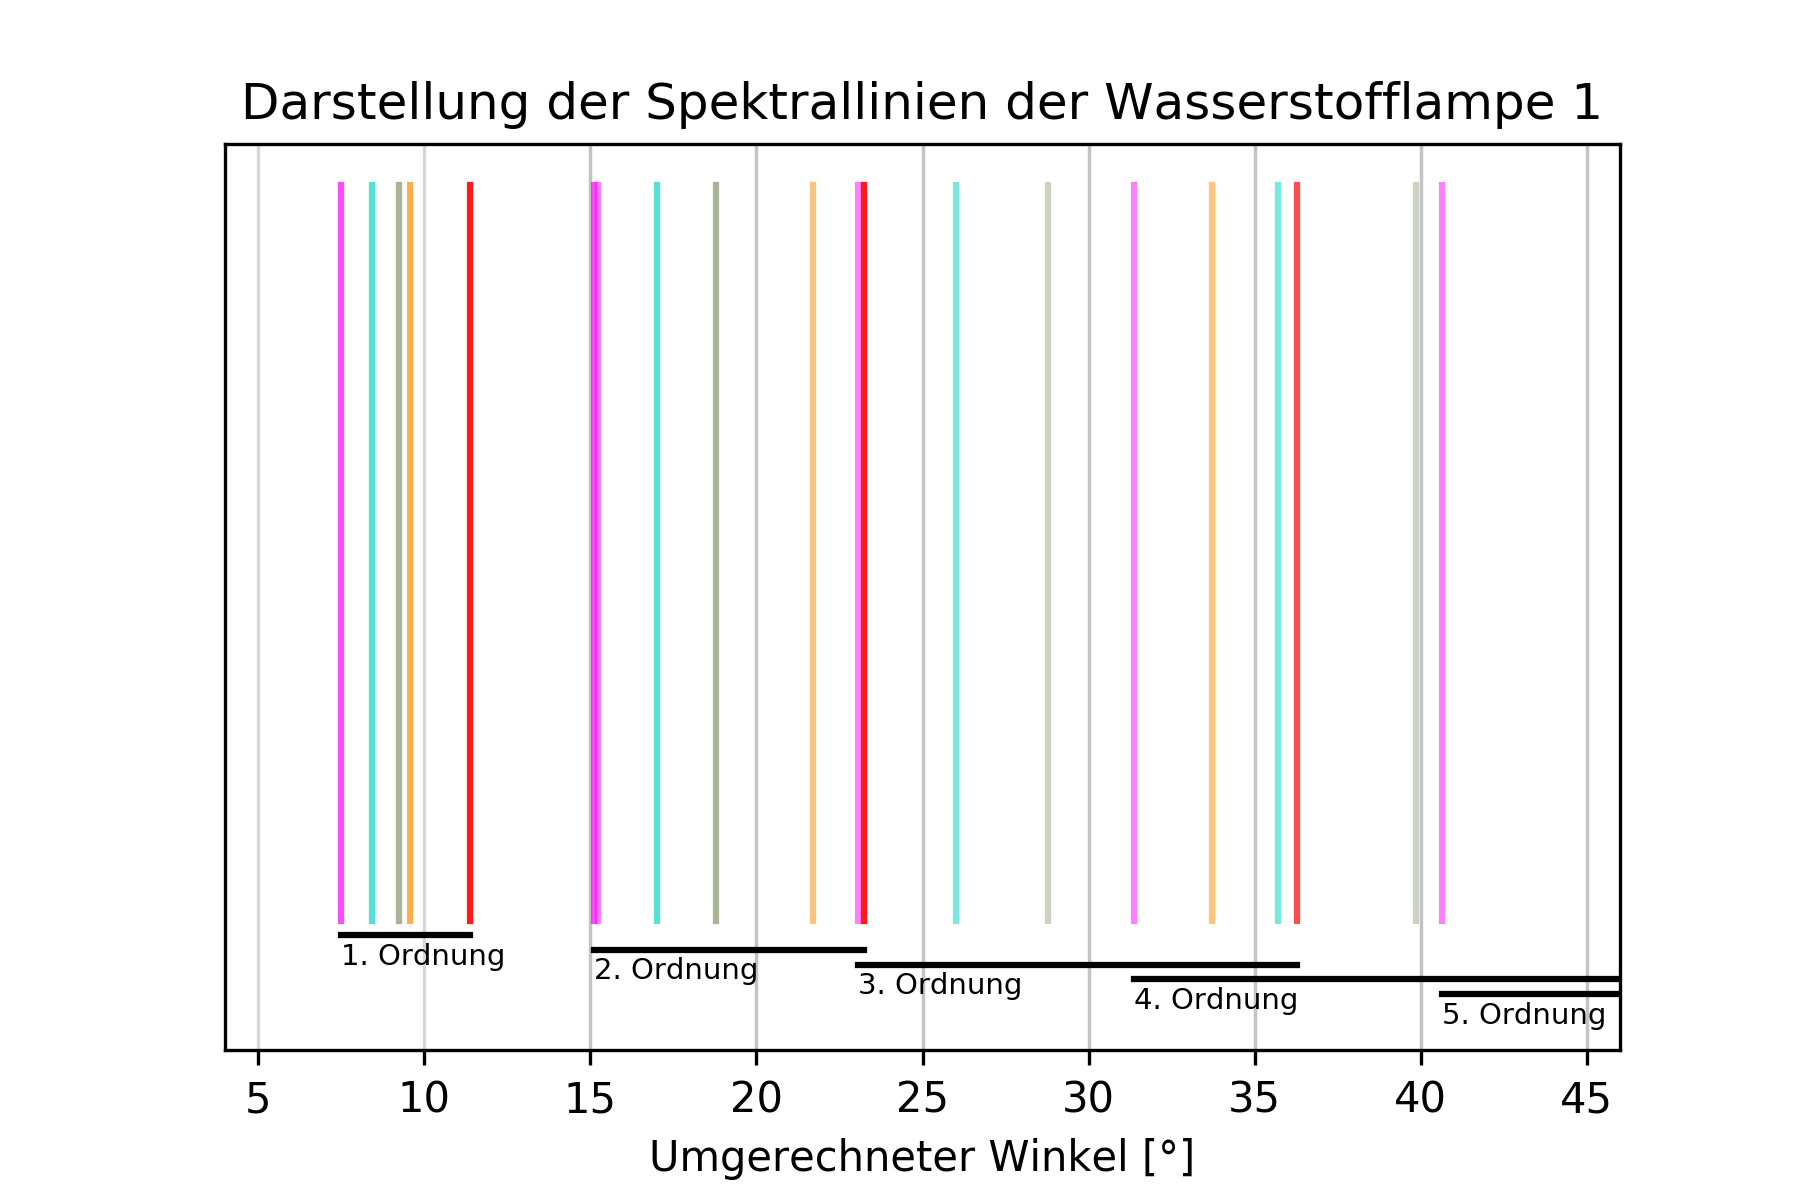
\includegraphics[width=1\textwidth]{Plots/HD_Linien_0.png}
\caption{ Erster Teil des Spektrums der Wasserstofflampe. }
\label{fig:H Lines 0}
\end{figure}

\begin{figure}[H]
\centering
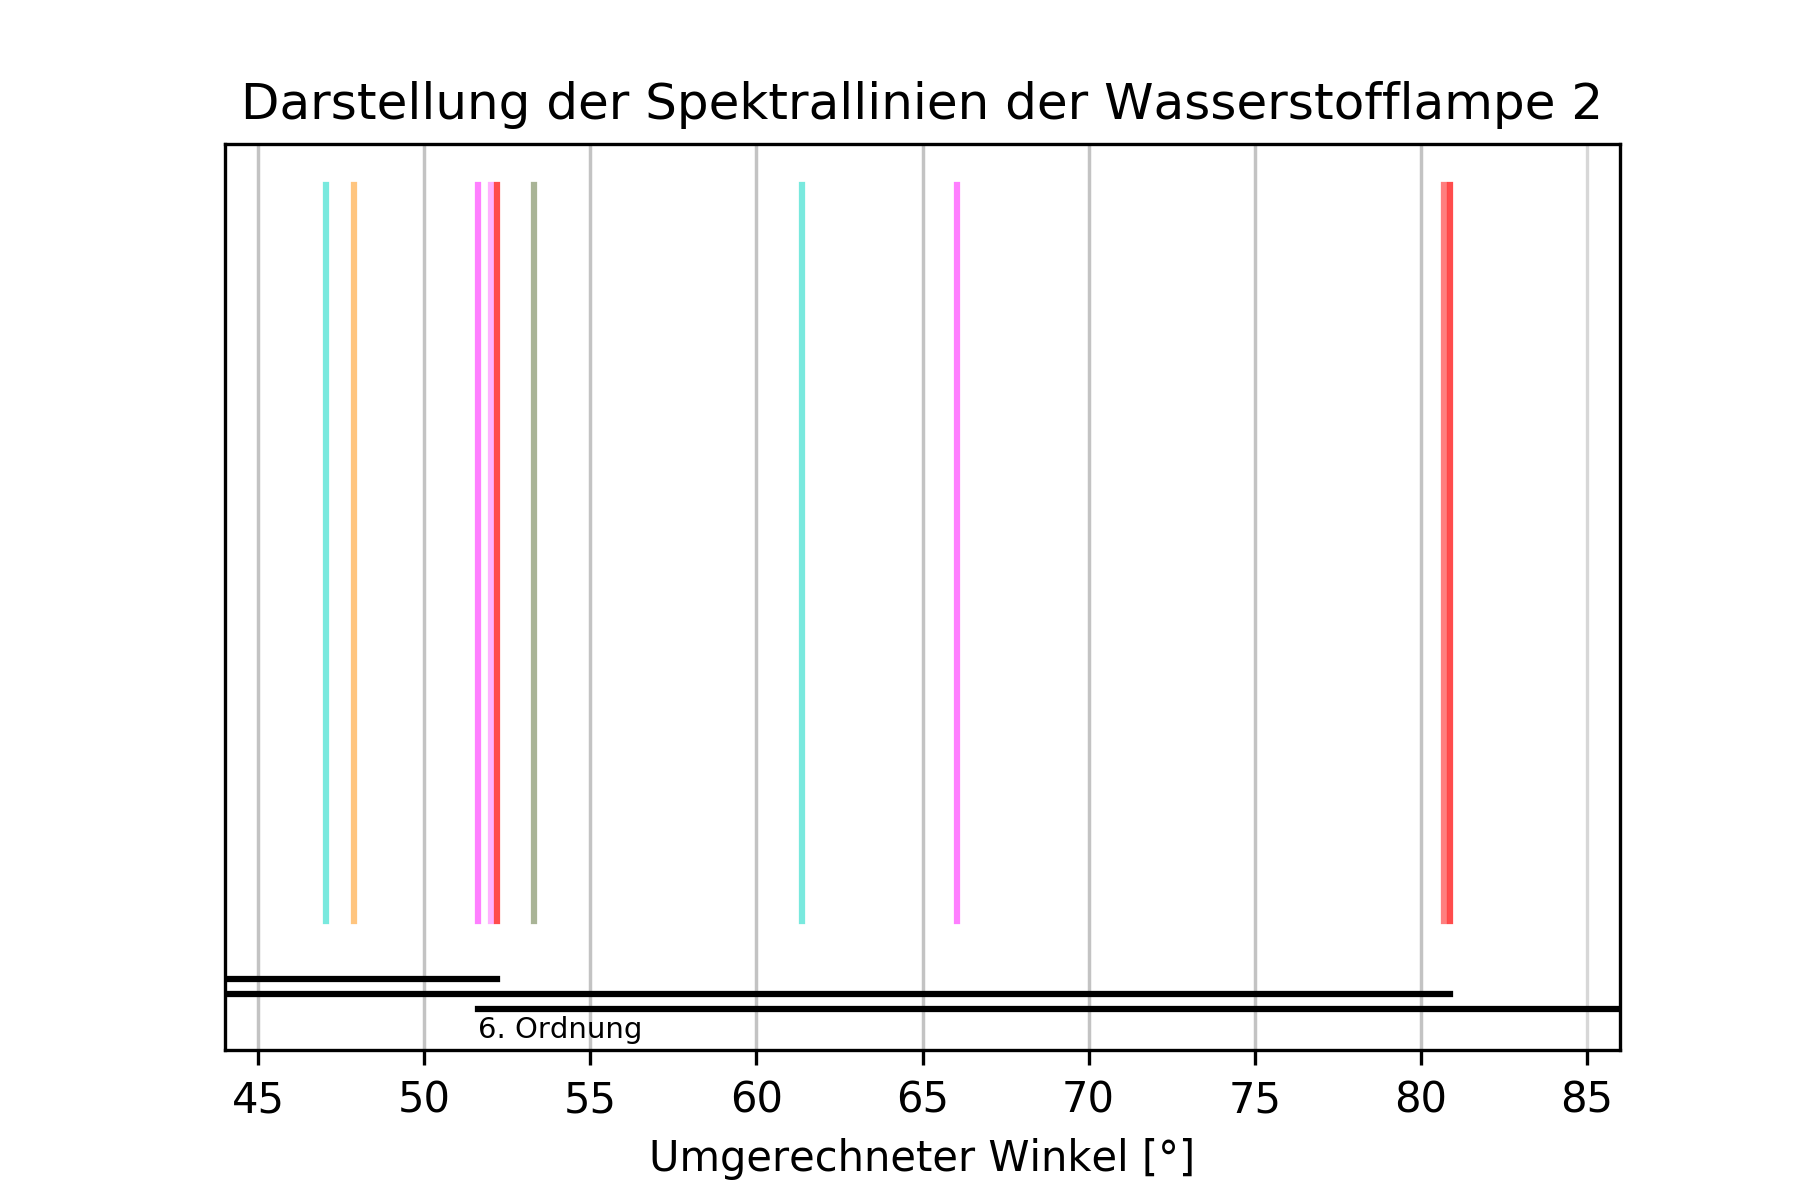
\includegraphics[width=1\textwidth]{Plots/HD_Linien_1.png}
\caption{ Zweiter Teil des Spektrums der Wasserstofflampe.}
\label{fig:H Lines 1}
\end{figure}

Hierbei erkennen wir deutlich die ersten drei Spektrallinien der Balmer Serie sowie zwei weitere Linien aus dem Sauerstoffspektrum. Stets in einer Ordnung wurden folgende Linien in absteigender Wellenlänge beobachtet:

\begin{table}[H]
	\centering
	\begin{tabular}{c|c|c|c|c|c}
		Linie & $H_\gamma$ & $H_\beta$ & $O$ & $O$ & $H_\alpha$ \\
		\hline
		Farbe & violett & türkis & gräulich grün & orange & rot \\
		\hline
		Wellenlänge [nm]  & 434 & 486 & 532 & 615 & 656 \\
	\end{tabular}
	\caption{Zuordnung der gemessenen Spektrallinien der Wasserstofflampe. Die Werte der Sauerstofflinien wurden aus Abbildung \ref{O Linien} abgelesen. }
\end{table}

Dabei konnten wir nur an drei Linien die Differenz der Wasserstoff- und Deuteriumlinien deutlich erkennen. Die violette Linie spaltete sich in den Ordnungen 2 und 6 sichtbar auf sowie dir rote am Ende des Spektrums in 5. Ordnung. Nachträglich wurden noch die türkisen Linien genauer betrachtet, jedoch ist deren Unterschied sehr gering gewesen.

%%%%%%%%%%%%%%%%%%%%%%%%%%%%%%%%%%%%% Grafik hier oder bei Auflösungsvermögen

% Gemittelte Wellenlöngen?

\subsubsection{Rydbergkonstante}
Durch die ermittelte Monochromatorkonstante und das Wasserstoffspektrum lassen sich nun die Rydbergkonstanten für $H$ und $D$ ermitteln. Dabei werden die drei genannten Doppellinien aufgeteilt und die einfachen Linien, sowie die türkisen, für beide Fits verwendet, da dort keine eindeutige Zuordnung möglich ist. Durch den schwereren Kern des Deuterium sind dessen Spektrallinien etwas energiereicher und somit nach links im Spektrum verschoben, da sie die kleinere Wellenlänge besitzen. 

\begin{figure}[H]
\centering
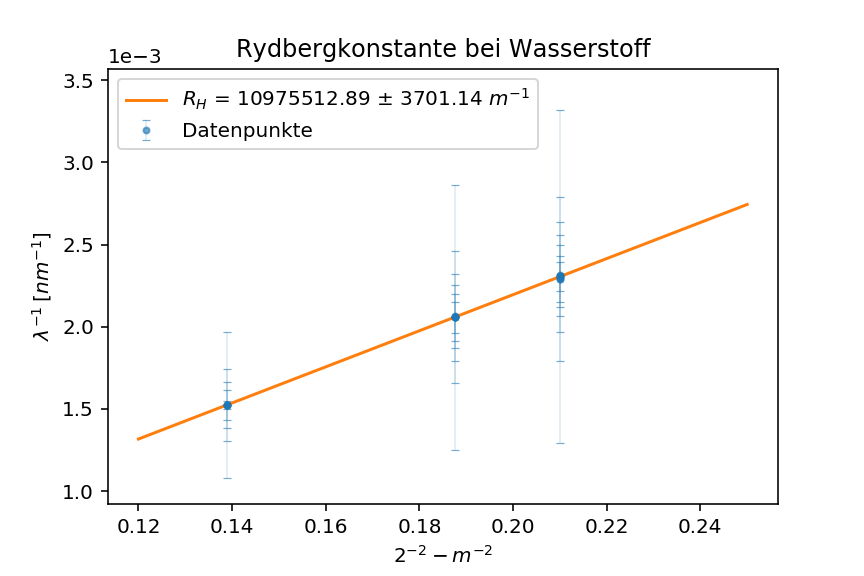
\includegraphics[width=1\textwidth]{Plots/R_H.png}
\caption{ Fit zur Bestimmung der Rydbergkonstante des Wasserstoff.}
\label{fig:Rydberg H}
\end{figure}

Es wurde hier ebenfalls wieder eine Gerade durch die Datenpunkte gefittet. Dabei wurden nach Gleichung (\ref{eq:rydberg}) das Inverse der Wellenlänge gegen den Faktor, welcher aus dem Energieunterschied zweier Energieniveaus ohne Feinstruktur hervorgeht, aufgetragen. Zuvor wurden die Wellenlängen mit unserer Monochromatorkonstante nach folgenden Gleichungen bestimmt:

\begin{equation}
\lambda = \frac{c}{n} sin(\delta) \:,\: \Delta\lambda = \frac{1}{n} \sqrt{(\Delta c \cdot sin(\delta))^2 + (c\cdot cos(\delta) )^2}
\end{equation}

\begin{figure}[H]
\centering
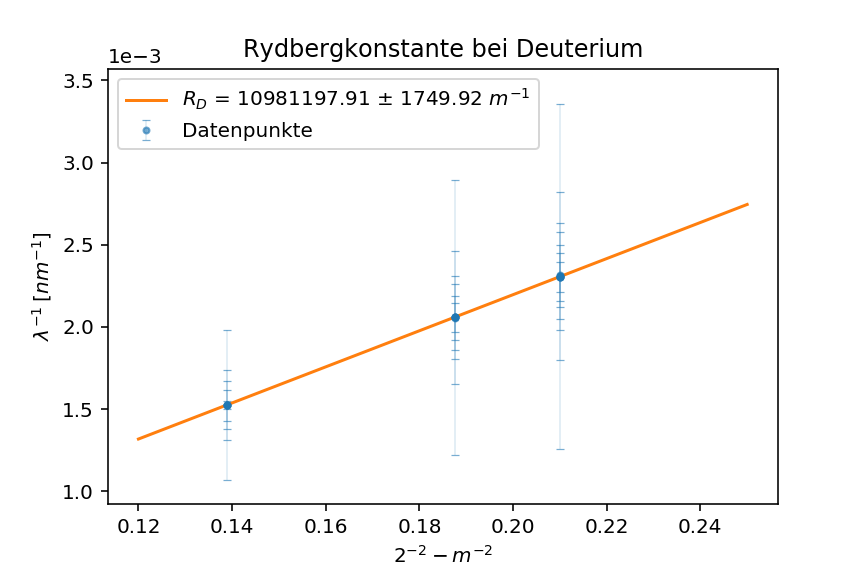
\includegraphics[width=1\textwidth]{Plots/R_D.png}
\caption{ Fit zur Bestimmung der Rydbergkonstante des Deuterium.}
\label{fig:Rydberg D}
\end{figure}

Die Resultate sind nun erstaunlich gut geworden im Vergleich mit dem Literaturwert $R_\infty = 10973731.57 m^{-1}$, welcher für einen unendlich schweren Kern gilt. Die folgende Tabelle verdeutlicht unsere Ergebnisse:

\begin{table}[H]
	\centering
	\begin{tabular}{c|c|c|c}
		  & Fit & Literaturwert & Relative Abweichung  \\
		\hline
		$R_H$ [$m^{-1}$]& $10\,975\,512.89\pm 3\,701.14$ & $10\,967\,758.34$ & $1.00071$ \\
		\hline
		$R_D$ [$m^{-1}$]& $10\,981\,888.31\pm 3\,046.17$ & $10\,970\,746.20$ & $1.00102$ \\
	\end{tabular}
	\caption{Übersicht unserer berechneten Rydbergkonstanten. Verglichen wird mit dem Literaturwert nach $R_i = R_\infty \frac{\mu_i}{m_e}$.}
\end{table}

Unsere Ergebnisse sind somit immer etwa um $0.1\%$ größer als der Literaturwert. Die Fehler, jene die Fitfunktion liefert, sind jedoch zu klein um den Literaturwert abzudecken. Es fehlen stets eine halbe bis ganze Größenordnung.

%Tabelle
%Gemittelte Wellenlängen und energien der Übergänge
%Rydbergconstante
%Irgendwas mit den Dopplelinien
\subsection{Fehlerdiskussion}

Zu beachten war, dass zwischen dem Winkel des Gitters und jenem welchen wir über das Maßband bestimmen konnten, ein Übersetzungsfaktor von 2 liegt. Für die Speltrallinien der Wasserstoff-Deuterium-Lampe haben wir im Raum einem Winkel von fast $180^\circ$ ausgenutzt, welches einer Gitterstellung von bis zu $90^\circ$ entspricht. Bei höheren Werten für $\delta$ gäbe es keine Linien zu sehen, da das Licht in die andere Richtung reflektiert wird. Ebenso kann die erneute Justierung des Spiegels nach $90^\circ$ zu einer Verschiebung im Winkel für die höheren Messungen geführt haben, jedoch wären dies nur wenige $cm$ und damit auch nur Verschiebungen vom wenigen Zehntel Grad, welche sehr gering sind.

Große Fehler in dem Abbildungen für die Rydbergkonstanten entstammen der Messung mit erster Ordnung. Dort wird aufgrund des $cos(\delta)$ der Fehlerwert für kleine Winkel nicht so stark gesenkt, im Vergleich zu den weiteren Messungen für große Winkel.
% Fit funktionen?

\subsection{Fazit}
% Confirmed: Bohr MOdel

\section{Anhang}

\begin{table}[H]
\centering
\begin{tabular}{|c|c|c|c|}
\hline
Ordnung & Farbe & $\delta$ & $\Delta\delta$ \\ \hline\hline
1 & violett & 8.09 & 0.06 \\ \hline
1 & blau & 8.19 & 0.06 \\ \hline
1 & oliv & 8.32 & 0.06 \\ \hline
1 & rot & 11.05 & 0.06 \\ \hline
2 & violett & 16.34 & 0.06 \\ \hline
2 & blau & 16.52 & 0.06 \\ \hline
2 & oliv & 16.83 & 0.06 \\ \hline
2 & rot & 22.49 & 0.06 \\ \hline
3 & violett & 24.96 & 0.06 \\ \hline
3 & blau & 25.22 & 0.06 \\ \hline
3 & oliv & 25.72 & 0.06 \\ \hline
3 & rot & 34.97 & 0.07 \\ \hline
4 & violett & 34.26 & 0.07 \\ \hline
4 & blau & 34.61 & 0.07 \\ \hline
4 & oliv & 35.34 & 0.07 \\ \hline
4 & rot & 50.37 & 0.08 \\ \hline
5 & violett & 44.7 & 0.07 \\ \hline
5 & blau & 45.25 & 0.07 \\ \hline
\hline
\end{tabular}
\caption{Daten zum Zinkspektrum.\label{Zn Data}}
\end{table}

\begin{table}[H]
\centering
\begin{tabular}{|c|c|c|c|}
\hline
Ordnung n & $\lambda$ [nm] & $sin(\delta)$ & $\Delta sin(\delta)$ \\ \hline\hline
1 & 468.0 & 0.1408 & 0.001 \\ \hline
1 & 472.2 & 0.1424 & 0.001 \\ \hline
1 & 481.1 & 0.1447 & 0.001 \\ \hline
1 & 636.2 & 0.1916 & 0.001 \\ \hline
2 & 468.0 & 0.2813 & 0.001 \\ \hline
2 & 472.2 & 0.2843 & 0.001 \\ \hline
2 & 481.1 & 0.2895 & 0.001 \\ \hline
2 & 636.2 & 0.3826 & 0.001 \\ \hline
3 & 468.0 & 0.4219 & 0.001 \\ \hline
3 & 472.2 & 0.4261 & 0.001 \\ \hline
3 & 481.1 & 0.434 & 0.001 \\ \hline
3 & 636.2 & 0.5732 & 0.001 \\ \hline
4 & 468.0 & 0.563 & 0.001 \\ \hline
4 & 472.2 & 0.5679 & 0.001 \\ \hline
4 & 481.1 & 0.5784 & 0.001 \\ \hline
4 & 636.2 & 0.7702 & 0.0008 \\ \hline
5 & 468.0 & 0.7034 & 0.0009 \\ \hline
5 & 472.2 & 0.7102 & 0.0009 \\ \hline
\hline \hline
1 & 589.3 & 0.1769 & 0.001 \\ \hline
2 & 589.3 & 0.36 & 0.001 \\ \hline
3 & 589.3 & 0.5316 & 0.001 \\ \hline
4 & 589.3 & 0.7084 & 0.0009 \\ \hline
\hline
\end{tabular}
\caption{Werte des Fits für die Gitterkonstante. Oben die Werte für Zink und unten Natrium. Gemittelte Wellenlänge der Doppellinie, da keine zusätzlichen Daten aufgenommen wurden.\label{c Data}}
\end{table}

\begin{figure}[H]
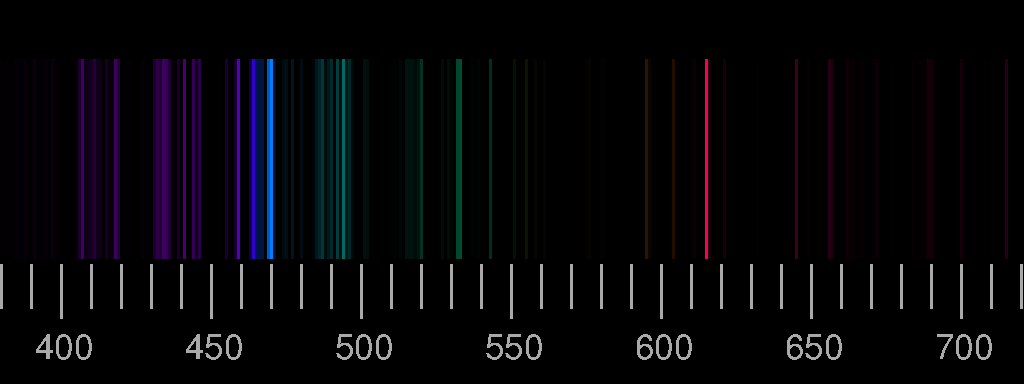
\includegraphics[width=1\textwidth]{Plots/spektO.png}
\caption{Spektrallinien von Sauerstoff. \cite{spektO}}
\label{O Linien}
\end{figure}

\begin{table}[H]
\centering
\begin{tabular}{|c|c|c|c|c|c|}
\hline
Ordnung & Farbe & $\delta$ & $\Delta\delta$ & $\lambda$ [nm] & $\Delta\lambda$ [nm] \\ \hline\hline
1 & violett & 7.5 & 0.06 & 433.57 & 197.6 \\ \hline
1 & türkis & 8.41 & 0.06 & 485.82 & 197.16 \\ \hline
1 & grau-grün & 9.24 & 0.06 & 533.37 & 196.72 \\ \hline
1 & orange & 9.56 & 0.06 & 551.68 & 196.54 \\ \hline
1 & rot & 11.39 & 0.06 & 656.0 & 195.38 \\ \hline
2 & violett & 15.11 & 0.06 & 432.94 & 96.21 \\ \hline
2 & violett & 15.23 & 0.06 & 436.3 & 96.15 \\ \hline
2 & türkis & 17.0 & 0.06 & 485.59 & 95.3 \\ \hline
2 & grau-grün & 18.77 & 0.06 & 534.42 & 94.35 \\ \hline
2 & orange & 21.72 & 0.06 & 614.64 & 92.58 \\ \hline
3 & violett & 23.07 & 0.06 & 433.88 & 61.12 \\ \hline
2 & rot & 23.24 & 0.06 & 655.35 & 91.57 \\ \hline
3 & türkis & 26.02 & 0.06 & 485.73 & 59.7 \\ \hline
3 & grau-grün & 28.79 & 0.06 & 533.25 & 58.22 \\ \hline
4 & violett & 31.37 & 0.07 & 432.29 & 49.63 \\ \hline
3 & orange & 33.71 & 0.07 & 614.51 & 64.48 \\ \hline
4 & türkis & 35.72 & 0.07 & 484.83 & 47.2 \\ \hline
3 & rot & 36.29 & 0.07 & 655.35 & 62.48 \\ \hline
4 & grau-grün & 39.87 & 0.07 & 532.35 & 44.62 \\ \hline
5 & violett & 40.64 & 0.07 & 432.69 & 35.29 \\ \hline
5 & türkis & 47.05 & 0.07 & 486.27 & 31.69 \\ \hline
4 & orange & 47.89 & 0.07 & 616.07 & 38.98 \\ \hline
6 & violett & 51.63 & 0.08 & 434.05 & 27.49 \\ \hline
6 & violett & 52.01 & 0.08 & 436.32 & 27.26 \\ \hline
4 & rot & 52.2 & 0.08 & 656.17 & 40.72 \\ \hline
5 & grau-grün & 53.29 & 0.08 & 532.59 & 31.77 \\ \hline
6 & türkis & 61.36 & 0.08 & 485.89 & 21.23 \\ \hline
7 & violett & 66.05 & 0.09 & 433.68 & 17.34 \\ \hline
5 & rot & 80.71 & 0.1 & 655.63 & 10.73 \\ \hline
5 & rot & 80.88 & 0.1 & 655.95 & 10.54 \\ \hline
\hline
\end{tabular}
\caption{Daten zum Wasserstoffspektrum.\label{H Data}}
\end{table}


\newpage
\begin{thebibliography}{}

\bibitem{skript} \begin{verbatim}
lectures__2006__ss06_FPraktikum__V17_20060907_BalmerSerie.pdf
\end{verbatim} (Begleitendes Skript zum Versuch 17: Balmer Serie)

\bibitem{spektO} \begin{verbatim}
https://www.itp.uni-hannover.de/fileadmin/arbeitsgruppen/zawischa/static_html/atome.html
\end{verbatim} 

\end{thebibliography}
\end{document}

